
%% bare_conf.tex
%% V1.4
%% 2012/12/27
%% by Michael Shell
%% See:
%% http://www.michaelshell.org/
%% for current contact information.
%%
%% This is a skeleton file demonstrating the use of IEEEtran.cls
%% (requires IEEEtran.cls version 1.8 or later) with an IEEE conference paper.
%%
%% Support sites:
%% http://www.michaelshell.org/tex/ieeetran/
%% http://www.ctan.org/tex-archive/macros/latex/contrib/IEEEtran/
%% and
%% http://www.ieee.org/

%%*************************************************************************
%% Legal Notice:
%% This code is offered as-is without any warranty either expressed or
%% implied; without even the implied warranty of MERCHANTABILITY or
%% FITNESS FOR A PARTICULAR PURPOSE! 
%% User assumes all risk.
%% In no event shall IEEE or any contributor to this code be liable for
%% any damages or losses, including, but not limited to, incidental,
%% consequential, or any other damages, resulting from the use or misuse
%% of any information contained here.
%%
%% All comments are the opinions of their respective authors and are not
%% necessarily endorsed by the IEEE.
%%
%% This work is distributed under the LaTeX Project Public License (LPPL)
%% ( http://www.latex-project.org/ ) version 1.3, and may be freely used,
%% distributed and modified. A copy of the LPPL, version 1.3, is included
%% in the base LaTeX documentation of all distributions of LaTeX released
%% 2003/12/01 or later.
%% Retain all contribution notices and credits.
%% ** Modified files should be clearly indicated as such, including  **
%% ** renaming them and changing author support contact information. **
%%
%% File list of work: IEEEtran.cls, IEEEtran_HOWTO.pdf, bare_adv.tex,
%%                    bare_conf.tex, bare_jrnl.tex, bare_jrnl_compsoc.tex,
%%                    bare_jrnl_transmag.tex
%%*************************************************************************

% *** Authors should verify (and, if needed, correct) their LaTeX system  ***
% *** with the testflow diagnostic prior to trusting their LaTeX platform ***
% *** with production work. IEEE's font choices can trigger bugs that do  ***
% *** not appear when using other class files.                            ***
% The testflow support page is at:
% http://www.michaelshell.org/tex/testflow/



% Note that the a4paper option is mainly intended so that authors in
% countries using A4 can easily print to A4 and see how their papers will
% look in print - the typesetting of the document will not typically be
% affected with changes in paper size (but the bottom and side margins will).
% Use the testflow package mentioned above to verify correct handling of
% both paper sizes by the user's LaTeX system.
%
% Also note that the "draftcls" or "draftclsnofoot", not "draft", option
% should be used if it is desired that the figures are to be displayed in
% draft mode.
%
\documentclass[conference]{IEEEtran}
% Add the compsoc option for Computer Society conferences.
%
% If IEEEtran.cls has not been installed into the LaTeX system files,
% manually specify the path to it like:
% \documentclass[conference]{../sty/IEEEtran}





% Some very useful LaTeX packages include:
% (uncomment the ones you want to load)


% *** MISC UTILITY PACKAGES ***
%
%\usepackage{ifpdf}
% Heiko Oberdiek's ifpdf.sty is very useful if you need conditional
% compilation based on whether the output is pdf or dvi.
% usage:
% \ifpdf
%   % pdf code
% \else
%   % dvi code
% \fi
% The latest version of ifpdf.sty can be obtained from:
% http://www.ctan.org/tex-archive/macros/latex/contrib/oberdiek/
% Also, note that IEEEtran.cls V1.7 and later provides a builtin
% \ifCLASSINFOpdf conditional that works the same way.
% When switching from latex to pdflatex and vice-versa, the compiler may
% have to be run twice to clear warning/error messages.






% *** CITATION PACKAGES ***
%
%\usepackage{cite}
% cite.sty was written by Donald Arseneau
% V1.6 and later of IEEEtran pre-defines the format of the cite.sty package
% \cite{} output to follow that of IEEE. Loading the cite package will
% result in citation numbers being automatically sorted and properly
% "compressed/ranged". e.g., [1], [9], [2], [7], [5], [6] without using
% cite.sty will become [1], [2], [5]--[7], [9] using cite.sty. cite.sty's
% \cite will automatically add leading space, if needed. Use cite.sty's
% noadjust option (cite.sty V3.8 and later) if you want to turn this off
% such as if a citation ever needs to be enclosed in parenthesis.
% cite.sty is already installed on most LaTeX systems. Be sure and use
% version 4.0 (2003-05-27) and later if using hyperref.sty. cite.sty does
% not currently provide for hyperlinked citations.
% The latest version can be obtained at:
% http://www.ctan.org/tex-archive/macros/latex/contrib/cite/
% The documentation is contained in the cite.sty file itself.






% *** GRAPHICS RELATED PACKAGES ***
%
\ifCLASSINFOpdf
   \usepackage[pdftex]{graphicx}
  % declare the path(s) where your graphic files are
  % \graphicspath{{../pdf/}{../jpeg/}}
  % and their extensions so you won't have to specify these with
  % every instance of \includegraphics
  \DeclareGraphicsExtensions{.pdf,.jpeg,.png}
\else
  % or other class option (dvipsone, dvipdf, if not using dvips). graphicx
  % will default to the driver specified in the system graphics.cfg if no
  % driver is specified.
  % \usepackage[dvips]{graphicx}
  % declare the path(s) where your graphic files are
  % \graphicspath{{../eps/}}
  % and their extensions so you won't have to specify these with
  % every instance of \includegraphics
  % \DeclareGraphicsExtensions{.eps}
\fi
% graphicx was written by David Carlisle and Sebastian Rahtz. It is
% required if you want graphics, photos, etc. graphicx.sty is already
% installed on most LaTeX systems. The latest version and documentation
% can be obtained at: 
% http://www.ctan.org/tex-archive/macros/latex/required/graphics/
% Another good source of documentation is "Using Imported Graphics in
% LaTeX2e" by Keith Reckdahl which can be found at:
% http://www.ctan.org/tex-archive/info/epslatex/
%
% latex, and pdflatex in dvi mode, support graphics in encapsulated
% postscript (.eps) format. pdflatex in pdf mode supports graphics
% in .pdf, .jpeg, .png and .mps (metapost) formats. Users should ensure
% that all non-photo figures use a vector format (.eps, .pdf, .mps) and
% not a bitmapped formats (.jpeg, .png). IEEE frowns on bitmapped formats
% which can result in "jaggedy"/blurry rendering of lines and letters as
% well as large increases in file sizes.
%
% You can find documentation about the pdfTeX application at:
% http://www.tug.org/applications/pdftex





% *** MATH PACKAGES ***
%
\usepackage[cmex10]{amsmath}
% A popular package from the American Mathematical Society that provides
% many useful and powerful commands for dealing with mathematics. If using
% it, be sure to load this package with the cmex10 option to ensure that
% only type 1 fonts will utilized at all point sizes. Without this option,
% it is possible that some math symbols, particularly those within
% footnotes, will be rendered in bitmap form which will result in a
% document that can not be IEEE Xplore compliant!
%
% Also, note that the amsmath package sets \interdisplaylinepenalty to 10000
% thus preventing page breaks from occurring within multiline equations. Use:
%\interdisplaylinepenalty=2500
% after loading amsmath to restore such page breaks as IEEEtran.cls normally
% does. amsmath.sty is already installed on most LaTeX systems. The latest
% version and documentation can be obtained at:
% http://www.ctan.org/tex-archive/macros/latex/required/amslatex/math/





% *** SPECIALIZED LIST PACKAGES ***
%
%\usepackage{algorithmic}
% algorithmic.sty was written by Peter Williams and Rogerio Brito.
% This package provides an algorithmic environment fo describing algorithms.
% You can use the algorithmic environment in-text or within a figure
% environment to provide for a floating algorithm. Do NOT use the algorithm
% floating environment provided by algorithm.sty (by the same authors) or
% algorithm2e.sty (by Christophe Fiorio) as IEEE does not use dedicated
% algorithm float types and packages that provide these will not provide
% correct IEEE style captions. The latest version and documentation of
% algorithmic.sty can be obtained at:
% http://www.ctan.org/tex-archive/macros/latex/contrib/algorithms/
% There is also a support site at:
% http://algorithms.berlios.de/index.html
% Also of interest may be the (relatively newer and more customizable)
% algorithmicx.sty package by Szasz Janos:
% http://www.ctan.org/tex-archive/macros/latex/contrib/algorithmicx/




% *** ALIGNMENT PACKAGES ***
%
\usepackage{array}
% Frank Mittelbach's and David Carlisle's array.sty patches and improves
% the standard LaTeX2e array and tabular environments to provide better
% appearance and additional user controls. As the default LaTeX2e table
% generation code is lacking to the point of almost being broken with
% respect to the quality of the end results, all users are strongly
% advised to use an enhanced (at the very least that provided by array.sty)
% set of table tools. array.sty is already installed on most systems. The
% latest version and documentation can be obtained at:
% http://www.ctan.org/tex-archive/macros/latex/required/tools/


% IEEEtran contains the IEEEeqnarray family of commands that can be used to
% generate multiline equations as well as matrices, tables, etc., of high
% quality.




% *** SUBFIGURE PACKAGES ***
\ifCLASSOPTIONcompsoc
  \usepackage[caption=false,font=normalsize,labelfont=sf,textfont=sf]{subfig}
\else
  \usepackage[caption=false,font=footnotesize]{subfig}
\fi
% subfig.sty, written by Steven Douglas Cochran, is the modern replacement
% for subfigure.sty, the latter of which is no longer maintained and is
% incompatible with some LaTeX packages including fixltx2e. However,
% subfig.sty requires and automatically loads Axel Sommerfeldt's caption.sty
% which will override IEEEtran.cls' handling of captions and this will result
% in non-IEEE style figure/table captions. To prevent this problem, be sure
% and invoke subfig.sty's "caption=false" package option (available since
% subfig.sty version 1.3, 2005/06/28) as this is will preserve IEEEtran.cls
% handling of captions.
% Note that the Computer Society format requires a larger sans serif font
% than the serif footnote size font used in traditional IEEE formatting
% and thus the need to invoke different subfig.sty package options depending
% on whether compsoc mode has been enabled.
%
% The latest version and documentation of subfig.sty can be obtained at:
% http://www.ctan.org/tex-archive/macros/latex/contrib/subfig/




% *** FLOAT PACKAGES ***
%
\usepackage{fixltx2e}
% fixltx2e, the successor to the earlier fix2col.sty, was written by
% Frank Mittelbach and David Carlisle. This package corrects a few problems
% in the LaTeX2e kernel, the most notable of which is that in current
% LaTeX2e releases, the ordering of single and double column floats is not
% guaranteed to be preserved. Thus, an unpatched LaTeX2e can allow a
% single column figure to be placed prior to an earlier double column
% figure. The latest version and documentation can be found at:
% http://www.ctan.org/tex-archive/macros/latex/base/


%\usepackage{stfloats}
% stfloats.sty was written by Sigitas Tolusis. This package gives LaTeX2e
% the ability to do double column floats at the bottom of the page as well
% as the top. (e.g., "\begin{figure*}[!b]" is not normally possible in
% LaTeX2e). It also provides a command:
%\fnbelowfloat
% to enable the placement of footnotes below bottom floats (the standard
% LaTeX2e kernel puts them above bottom floats). This is an invasive package
% which rewrites many portions of the LaTeX2e float routines. It may not work
% with other packages that modify the LaTeX2e float routines. The latest
% version and documentation can be obtained at:
% http://www.ctan.org/tex-archive/macros/latex/contrib/sttools/
% Do not use the stfloats baselinefloat ability as IEEE does not allow
% \baselineskip to stretch. Authors submitting work to the IEEE should note
% that IEEE rarely uses double column equations and that authors should try
% to avoid such use. Do not be tempted to use the cuted.sty or midfloat.sty
% packages (also by Sigitas Tolusis) as IEEE does not format its papers in
% such ways.
% Do not attempt to use stfloats with fixltx2e as they are incompatible.
% Instead, use Morten Hogholm'a dblfloatfix which combines the features
% of both fixltx2e and stfloats:
%
% \usepackage{dblfloatfix}
% The latest version can be found at:
% http://www.ctan.org/tex-archive/macros/latex/contrib/dblfloatfix/




% *** PDF, URL AND HYPERLINK PACKAGES ***
%
%\usepackage{url}
% url.sty was written by Donald Arseneau. It provides better support for
% handling and breaking URLs. url.sty is already installed on most LaTeX
% systems. The latest version and documentation can be obtained at:
% http://www.ctan.org/tex-archive/macros/latex/contrib/url/
% Basically, \url{my_url_here}.




% *** Do not adjust lengths that control margins, column widths, etc. ***
% *** Do not use packages that alter fonts (such as pslatex).         ***
% There should be no need to do such things with IEEEtran.cls V1.6 and later.
% (Unless specifically asked to do so by the journal or conference you plan
% to submit to, of course. )


% correct bad hyphenation here
\hyphenation{op-tical net-works semi-conduc-tor}
\usepackage{epstopdf}

\begin{document}
%
% paper title
% can use linebreaks \\ within to get better formatting as desired
% Do not put math or special symbols in the title.
\title{Event-based Household Energy Consumption Disaggregation of Individual Appliances}


% author names and affiliations
% use a multiple column layout for up to three different
% affiliations
\author{\IEEEauthorblockN{Michael Shell}
\IEEEauthorblockA{School of Electrical and\\Computer Engineering\\
Georgia Institute of Technology\\
Atlanta, Georgia 30332--0250\\
Email: http://www.michaelshell.org/contact.html}
\and
\IEEEauthorblockN{Homer Simpson}
\IEEEauthorblockA{Twentieth Century Fox\\
Springfield, USA\\
Email: homer@thesimpsons.com}
\and
\IEEEauthorblockN{James Kirk\\ and Montgomery Scott}
\IEEEauthorblockA{Starfleet Academy\\
San Francisco, California 96678-2391\\
Telephone: (800) 555--1212\\
Fax: (888) 555--1212}}

% conference papers do not typically use \thanks and this command
% is locked out in conference mode. If really needed, such as for
% the acknowledgment of grants, issue a \IEEEoverridecommandlockouts
% after \documentclass

% for over three affiliations, or if they all won't fit within the width
% of the page, use this alternative format:
% 
%\author{\IEEEauthorblockN{Michael Shell\IEEEauthorrefmark{1},
%Homer Simpson\IEEEauthorrefmark{2},
%James Kirk\IEEEauthorrefmark{3}, 
%Montgomery Scott\IEEEauthorrefmark{3} and
%Eldon Tyrell\IEEEauthorrefmark{4}}
%\IEEEauthorblockA{\IEEEauthorrefmark{1}School of Electrical and Computer Engineering\\
%Georgia Institute of Technology,
%Atlanta, Georgia 30332--0250\\ Email: see http://www.michaelshell.org/contact.html}
%\IEEEauthorblockA{\IEEEauthorrefmark{2}Twentieth Century Fox, Springfield, USA\\
%Email: homer@thesimpsons.com}
%\IEEEauthorblockA{\IEEEauthorrefmark{3}Starfleet Academy, San Francisco, California 96678-2391\\
%Telephone: (800) 555--1212, Fax: (888) 555--1212}
%\IEEEauthorblockA{\IEEEauthorrefmark{4}Tyrell Inc., 123 Replicant Street, Los Angeles, California 90210--4321}}




% use for special paper notices
%\IEEEspecialpapernotice{(Invited Paper)}




% make the title area
\maketitle

% As a general rule, do not put math, special symbols or citations
% in the abstract
\begin{abstract}
	Even with advances in smart grid technology and a growing demand for cost-effective  energy consumption, detailed information about energy usage is often not available for residential electricity consumers. One reason is that household energy usage is monitored at no more than a single point by the utility, only providing information on the aggregate power consumption.  In this paper, we attempt to disaggregate  energy usage data into specific appliances from single-point sensing measurements.  Our method involves extracting turn-on and turn-off signature windows from time-series real and reactive power data to obtain transient characteristics of each appliance.  We focus on determining the appropriate window size for each appliance in order to capture unique signatures.  We present the results of our approach on a publicly available dataset.
\end{abstract}

% no keywords




% For peer review papers, you can put extra information on the cover
% page as needed:
% \ifCLASSOPTIONpeerreview
% \begin{center} \bfseries EDICS Category: 3-BBND \end{center}
% \fi
%
% For peerreview papers, this IEEEtran command inserts a page break and
% creates the second title. It will be ignored for other modes.
\IEEEpeerreviewmaketitle



\section{Introduction}
%In this section, we provide the motivation and a brief description of the project.  A short discussion of related work in this area, including the methodology of previous competition winners is also provided.  This is followed by an overview of our approach, description of the raw data, and evaluation method.

The objective of residential non-intrusive load monitoring (NILM) is to monitor the major loads in a home from a single-point.  The alternative is to monitor each appliance individually, however, this scheme typically adds significant cost. Therefore, the challenge with NILM is to accurately disaggregate household energy consumption into the individual appliance level with data from single-point measurements.  

Prior research in the area of NILM has focused on the use of aggregate power consumption patterns as features to identify what appliance is being used and how much energy it is consuming. For example, the authors in \cite{mit} discuss various approaches in NILM, including detecting changes in steady-state power measurements and characterizing them as different events. Some challenges reported by the authors include different loads not exhibiting unique signatures in the 2D feature space and the difficulty in determining steady-state features due to turn-on transient noise.  Some recommended advanced techniques are to include the 3rd order harmonics as a feature and using turn-on transients for event detection.  The methodology in [2] and [3] follows a similar strategy, however, the training and test data are manually generated, resulting in a clean dataset that may not be representative of real household energy usage patterns.  Furthermore, the classification can become challenging if the number of appliances in the home is large. Additionally, the signature of some appliances may drift or vary over time due to operating conditions and the mode in which they are used. 

In this paper, we present a method that focuses on extracting turn-on and turn-off signature windows to obtain transient characteristics of each appliance.  The transient characteristics are observed from the difference of two moving average windows from time-series real and reactive power data.  We focus on determining the appropriate window length for each appliance in order to capture unique signatures.  We present the results of our approach using a publicly available dataset from the Belkin Energy Disaggregation Competition on kaggle.com \cite{Kaggle}. The dataset and methodology are described in detail in Section \ref{sec:dataMethod}.  Section \ref{sec:training} describes the approach for extracting signature windows for each appliance from the training data. Section \ref{sec:cv} describes the cross-validation procedure using the training data.  Section \ref{sec:test} describes application of our approach to the test data.  Finally, Section \ref{sec:concl} discusses results and ideas for future work.
%
%The goal of this paper is to document our approach and share insights and conclusions regarding household energy consumption disaggregation that we observed throughout the project. 

\section{Data and Methodology}\label{sec:dataMethod}
%The objective is this.... because of this and the dataset, our methodology is specifically chosen for ...This section provides an overview of the dataset and a description of our methodology. 



Because the dataset is representative of real world appliance usage data, and that we are trying to fine detect multiple appliances and not just major ones, we have chosen a specific methodology.  If we are just detecting major appliances a different methodology can be used.  Strategy is to detect when and appliance turns on and turns off as opposed to steady state characteristics.  Out of 40 appliances per home, only a few exhibit steady state features that allow discrimination from background noise or other appliances.  

\subsection{Dataset}
%Show visualizations
%-data description
%-training data
%-figures show differences domain/power domain
%	- explain reason for looking in difference domain
%	- test data-multiple devices, and steady state, no changes
%	-goal is to detect events on/off
%	-for example, constant power loads, show no change, eg. light
%	-needed to correct time stamps in order to accurately determine signature windows

In this paper, we utilize the complete dataset available from kaggle.com, provided by Belkin Energy \cite{Kaggle}.  The dataset is publicly available on the competition website and contains the first five harmonics of rms voltage and current on two phases for four households (labeled H1-H4),consisting of both training and testing datasets.  The dataset also contains high frequency noise (EMI) data for each household, but is not required with our approach. The training data consists of manually generated power consumption for each appliance at each home.  These typically consist of only one appliance switched on at a time, although background noise is present from untagged appliances.  Table \ref{table:dataset} shows the number of distinct appliances in each home an the number of training and test datasets provided.  Tagging labels in the training data are also provided by Belkin, however, these are not precise enough to correctly identify device on and off times. An example of the data from Home H2 is shown in Fig.\ref{fig:traintest}.  A discussion for tagging label correction is presented in Section \ref{sec:training}.   The observations recorded in each training and testing dataset cover approximately 24 hours.  

\begin{figure}[!t]	
	\centering
	\subfloat[Training]{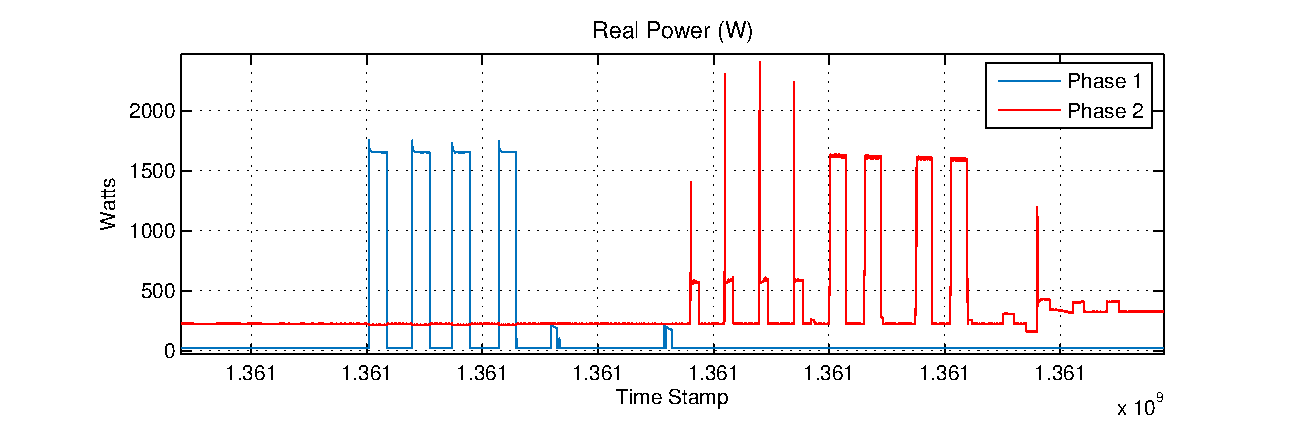
\includegraphics[width=2.5in]{fig/exTrain.eps}
		\label{fig:event1ml}}
	\hfil
	\subfloat[Test]{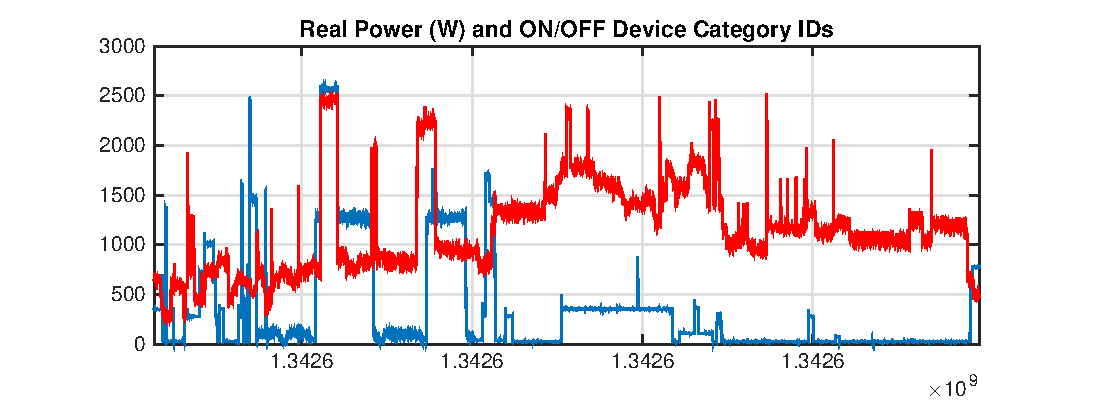
\includegraphics[width=2.5in]{fig/exTestH2_1.eps}
		\label{fig:event2ml}}
	%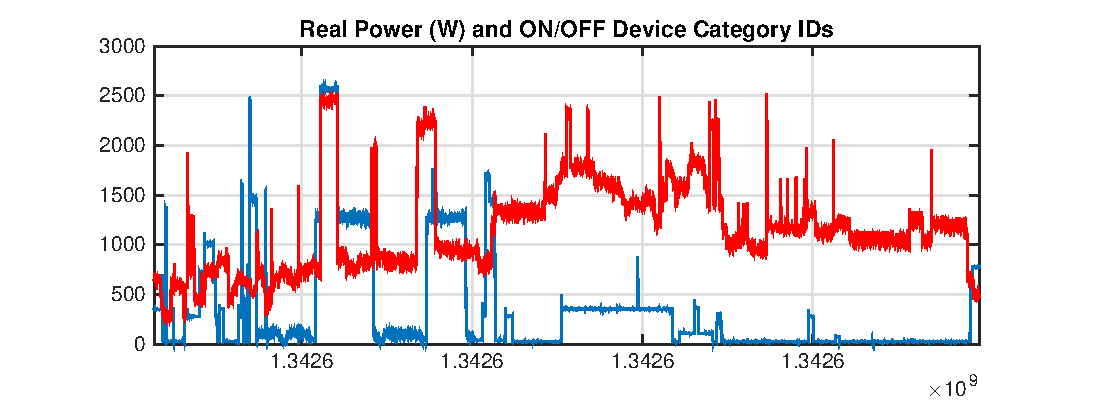
\includegraphics[width=3.5in]{fig/exTestH2_1.eps}
	\caption{Example of (a) training and (b) test data from Home 4.} 
	\label{fig:traintest}
\end{figure}

%For each home, the datasets include the first 5 harmonics of voltage and current measurements the FFT of the high frequency noise (captured every 1.0667 seconds).  The sampling rate is $f_s$ = 2 Mhz, which results in an FFT resolution of $f_r$ = 244.14 Hz. The dataset for each home is composed of several files.  For example, the data for H4 contains two training datasets and four testing datasets. The size and description of the files associated with each training and testing dataset are detailed in the tables below.

%\begin{table}[h]
%	\caption{Example of Data Files for Each Training and Testing Dataset}\label{files}
%	\begin{center}
%		%\vskip -5pt
%		\begin{tabular}{|l|l|l|}\hline
%			\textbf{File name} & \textbf{Description} & \textbf{Data Size}\\
%			\hline
%			HF & spectrogram of high frequency noise & 4096 $\times$ 81000\\
%			\hline
%			
%			TimeTicksHF &  UNIX timestamps corresponding to the HF & 81000$\times$1\\
%			\hline
%			
%			LF1V & fundamental and first 5 harmonics of 60Hz voltage of Phase-1. & 517067$\times$6\\
%			\hline
%			
%			LF1I & fundamental and first 5 harmonics of 60Hz current of Phase-1. & 517067$\times$6\\
%			\hline
%			
%			TimeTicks1 & UNIX timestamps corresponding to Phase-1 current and voltage. & 517067$\times$1\\
%			\hline
%			
%			LF2V & fundamental and first 5 harmonics of 60Hz voltage of Phase-2. &  517066$\times$6\\
%			\hline
%			
%			LF2I & fundamental and first 5 harmonics of 60Hz current of Phase-2. & 517066$\times$6\\
%			\hline
%			
%			Timeticks2 & UNIX timestamps corresponding to Phase-2 current and voltage. &  517066$\times$1\\
%			\hline
%			
%			TaggingInfo & labels for training purposes (For Training Data only) & 35$\times$4 \\
%			\hline
%		\end{tabular}
%	\end{center}
%\end{table}


\begin{table}[h!]
	\renewcommand{\arraystretch}{1.3}
	\caption{Number of Distinct Appliances and Datasets for Each Home}\label{classes}
	\label{table:dataset}
	\centering
	\begin{tabular}{p{1.5cm}||p{1.5cm}||p{1.5cm}||p{1.5cm}}
		\hline 
		\textbf{Home No.} & \textbf{Appliances} &\textbf{Training Sets} &\textbf{Test Sets}\tabularnewline
		\hline 
		\hline 
		H1 & 38 & 6 & 4\tabularnewline
		\hline 
		H2 & 37 & 4 & 4\tabularnewline
		\hline 
		H3 & 37 & 3 & 4\tabularnewline
		\hline 
		H4 & 36 & 2 & 4\tabularnewline
		\hline 
	\end{tabular}
\end{table}


\subsection{Methodology}

-explain methodology
- voltage/current harmonics to P/Q to differences to distances
-and why we use this approach
-include block diagram
-goal is to automate, this task can be done manually, but too tedious
-compare to previous and to data mining methods, ours is more interpretable
-ability for real time processing


\begin{figure}[!t]
	\centering
	\subfloat[]{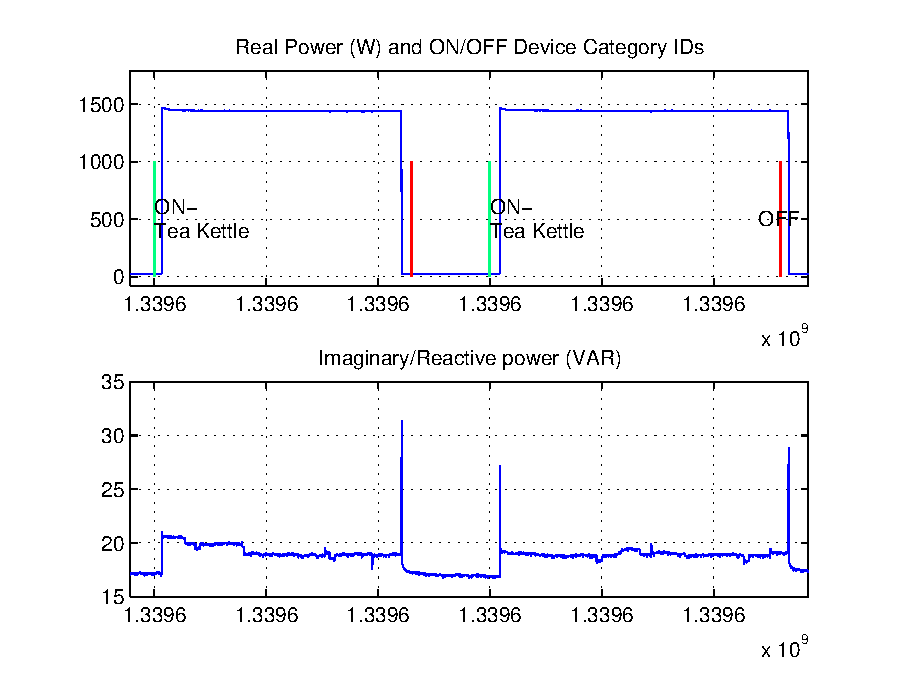
\includegraphics[width=1.7in]{fig/kettle.eps}
		\label{fig:event1}}
	\subfloat[]{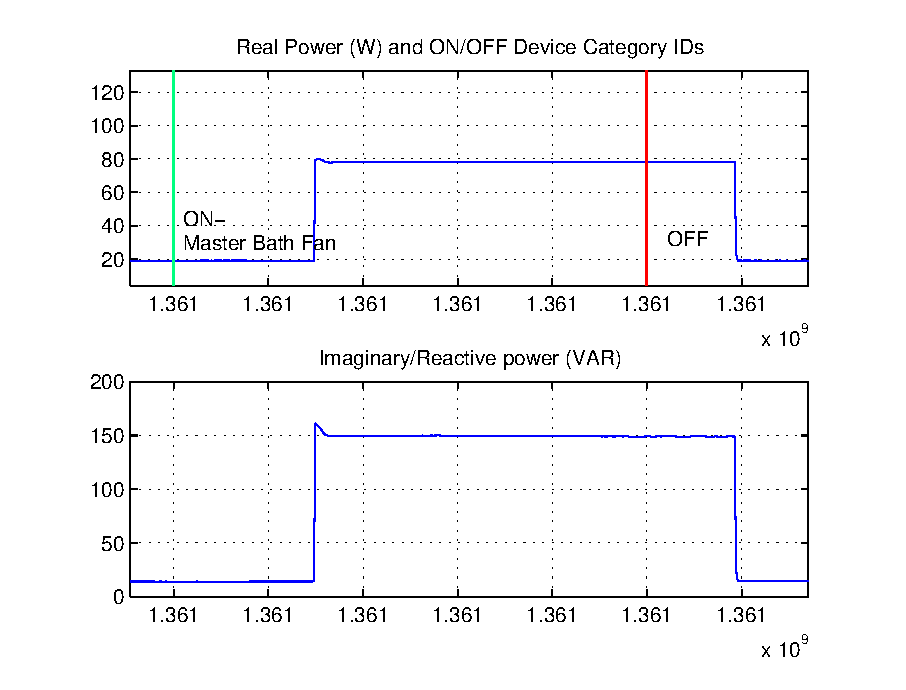
\includegraphics[width=1.7in]{fig/fan.eps}
		\label{fig:event2}}
	\hfill
	\subfloat[]{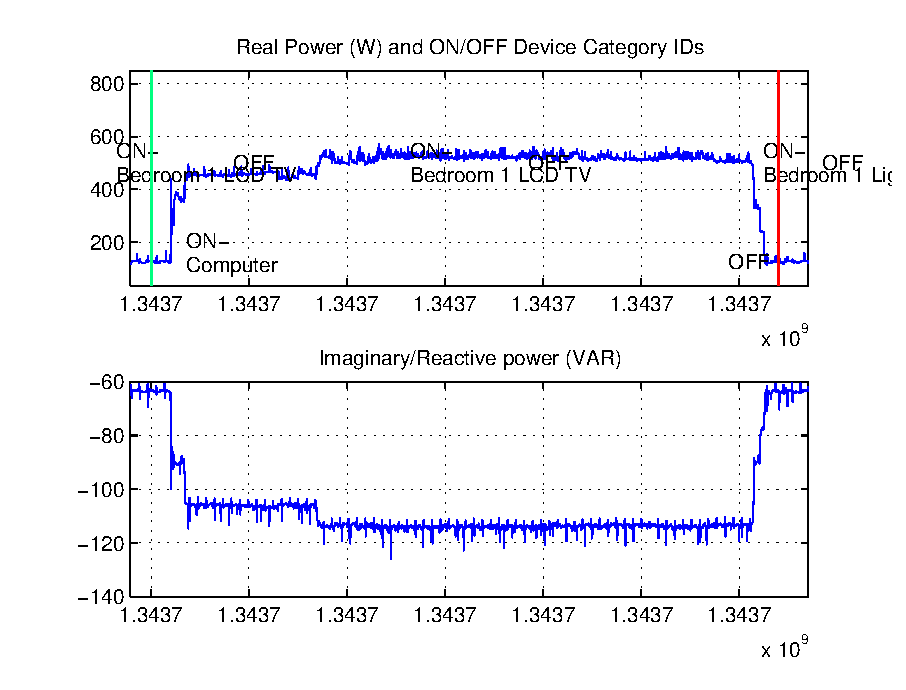
\includegraphics[width=1.7in]{fig/computer1.eps}
		\label{fig:event1}}
	\subfloat[]{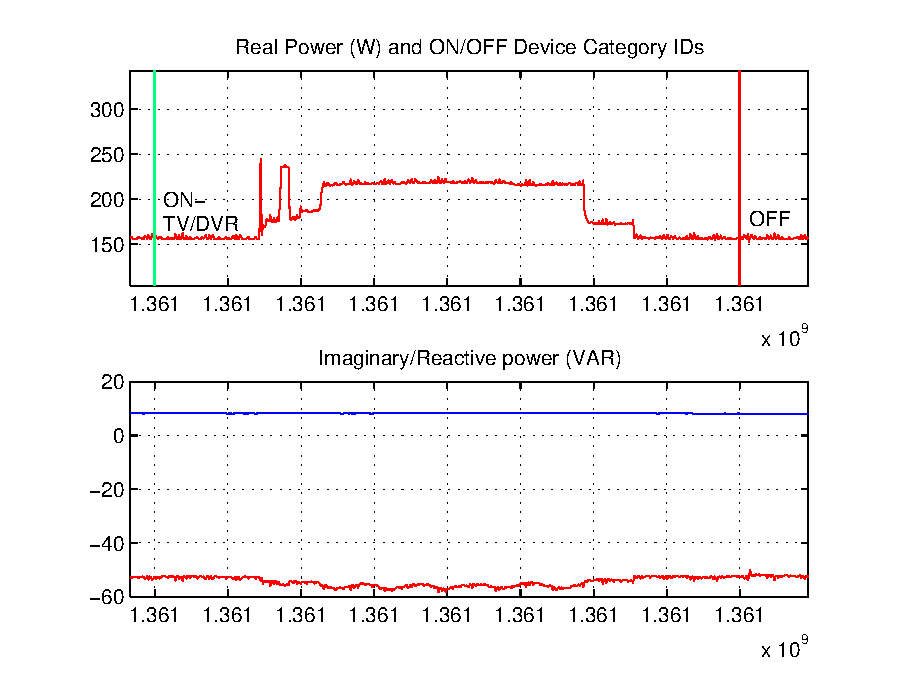
\includegraphics[width=1.7in]{fig/TV.eps}
		\label{fig:event2}}
	\hfill
	\subfloat[]{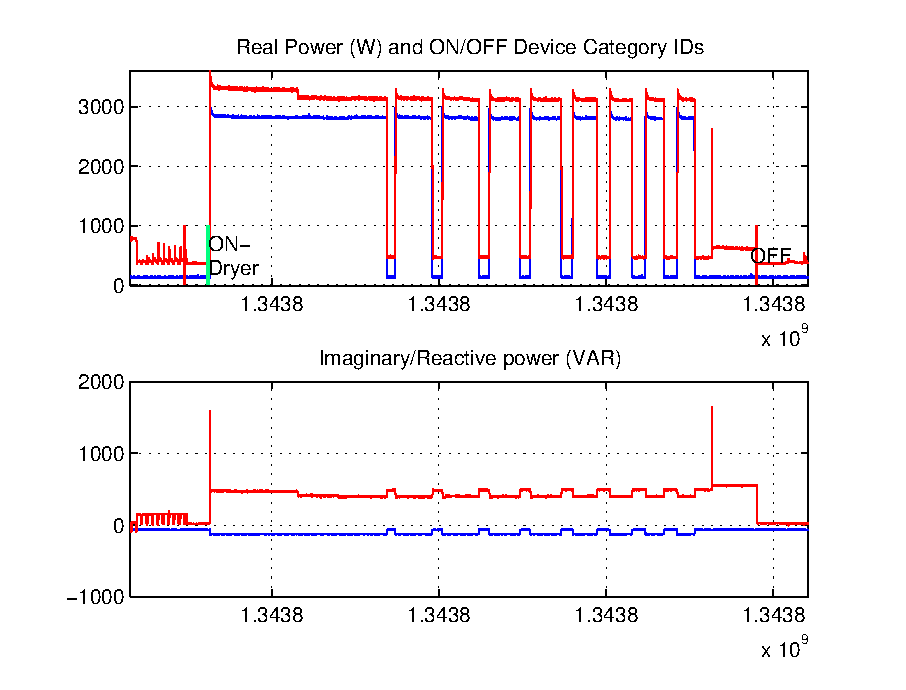
\includegraphics[width=1.7in]{fig/dryer.eps}
		\label{fig:event1}}
	\subfloat[]{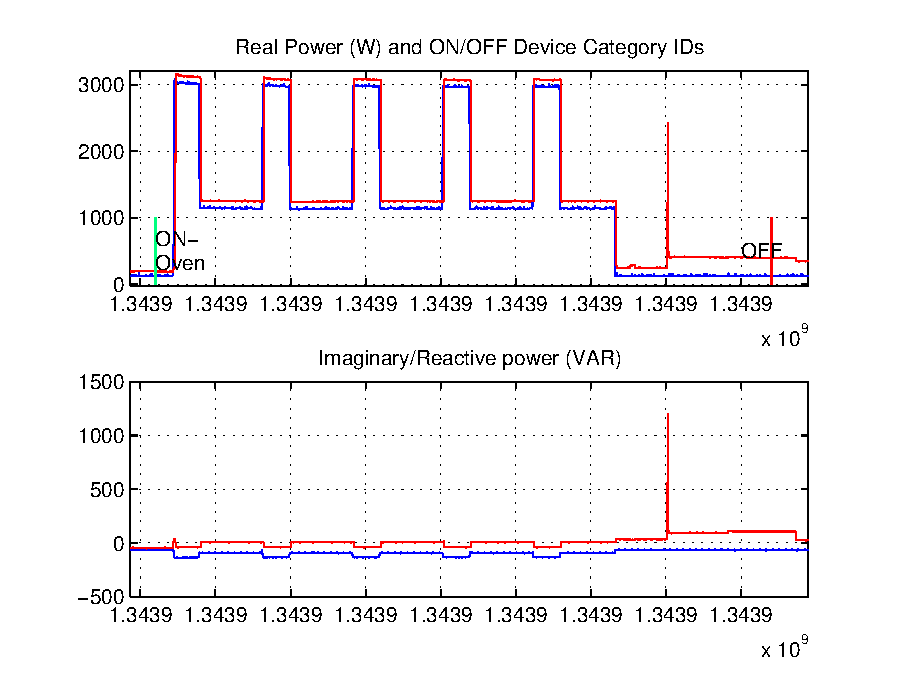
\includegraphics[width=1.7in]{fig/oven.eps}
		\label{fig:event2}}
	\caption{Load Types (a) Tea Kettle, (b) Master Bath Fan, (c) Computer, (d) TV, (e) Dryer, (f) Oven.}
	\label{fig:demon}
\end{figure}	

\section{Training - Signature Window Extraction}
This section concentrates on extracting the signature windows by using the real and the reactive power differences.  In particular, two ON/OFF signature windows are trained for each event of the appliances at each Home.  The following sections describe training signature windows depending on the shape of the load.  

\subsection{Load Types}
First, the appliances are categorized into three load types based on its shape.  The types include rectangular, non-rectangular, and cyclic loads.  
\begin{enumerate}
\item{Rectangular loads:} These type of loads consumes constant power when operating.  The load shapes are rectangular.  They include resistive loads, such as lights, heaters, and kettle, and reactive loads such as fans.  A short duration window consisting of the real and the reactive power differences are used to detect these loads.
\item{Non-rectangular loads:} These type of loads have a longer transient characteristics when turning on.  They include computers and TVs.  These type of loads require longer window length than the rectangular loads.
\item{Cyclical loads:} - These type of loads change it's shape depending on the cycle of their operation.  Dryer, oven, and washers are included in this category.  Two approaches are suggested to detect these type of loads; using multiple windows or detecting a notable landmark during the operation.
\end{enumerate}

\subsection{Smoothed Power Differences}
Now to train the windows, the real and the reactive power differences are calculated from two moving average windows.  The smoothed difference $S(n)$ is defined as,
\begin{equation}
S(n) = \frac{1}{N}\sum_{k=0}^{N}P(n-k) - \frac{1}{N}\sum_{k=N+D}^{2N+D}P(n-k)
\end{equation}
where $N$ is the window size and $D$ is the distance between the two windows. 
It should be noted that if shorter window size is used, it is easier to distinguish events from other events happening at the same incidence.  However, the detector becomes less robust to noise.

\begin{figure}[!t]
	\centering
	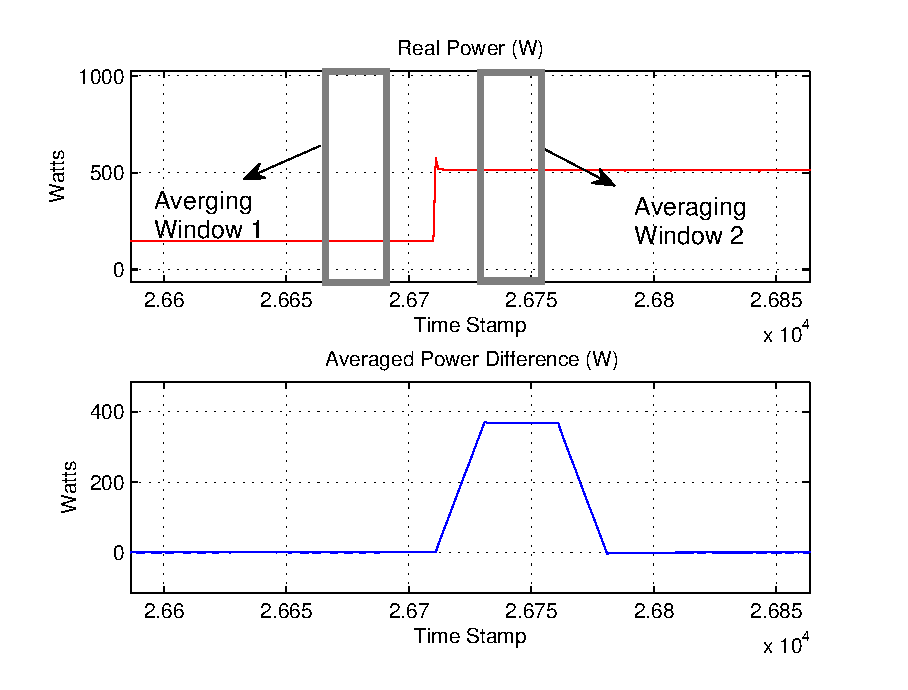
\includegraphics[width=3.5in]{fig/maw.eps}
	\caption{Two Moving Average Windows.}
	\label{fig:maw}
\end{figure}

Using the power difference,  the mismatches in the tagging info and the actual event index are corrected.  A threshold for the real power difference is set to indicate whether an event occurred, (event occurred if $|S(n)| >$ threshold).  Then this corrected indexes are used as the actual event index instead of the tagging info provided.  On the top plot of Fig. \ref{fig:tagging}, the tagging info of the master room lights do not align with the actual event incidence.  The red markers in the bottom plot shows when the power difference is greater than the threshold and this index is used as the corrected tagging info.  It should be noted that we discarded some appliances that consumes very small real or reactive power.  For these appliances, using real and reactive power differences will rather cause more false alarms in the test data due to the effects of the noises. 

\begin{figure}[!t]
	\centering
	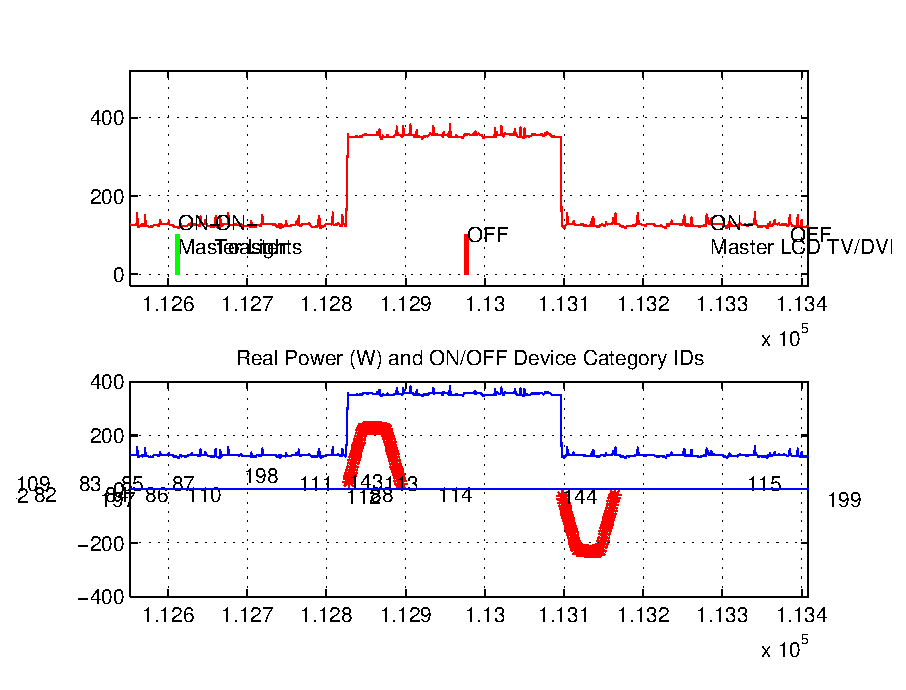
\includegraphics[width=3.5in]{fig/masterlights.eps}
	\caption{Tagging Info Correction.}
	\label{fig:tagging}
\end{figure}
	
<<<<<<< HEAD
\subsection{Signature Window Extraction}
After taking the power differences, the next stop is to extract the signatures for on-events and off-events. The windows are extracted starting from the corrected tagging info until the real and reactive power waveforms reach steady-state.  The power differences will increase to the rated power consumption of the appliance and decrease to zero, as shown in Fig. \ref{fig:maw}.

If an appliance has an longer transient characteristics (non-rectangular load shapes), longer window size is used to detect event.  For example, consider the dining room light and the laptop charger profile shown in Fig. \ref{fig:windowlength}.  Both the appliances consumes about 38 Watts at event incidence.  However, laptop charger then spends additional 38 Watts to fully turn on.  Therefore, longer window lengths are used to detect laptop charger than in detecting the dining room lights. 

\begin{figure}[!t]
	\centering
	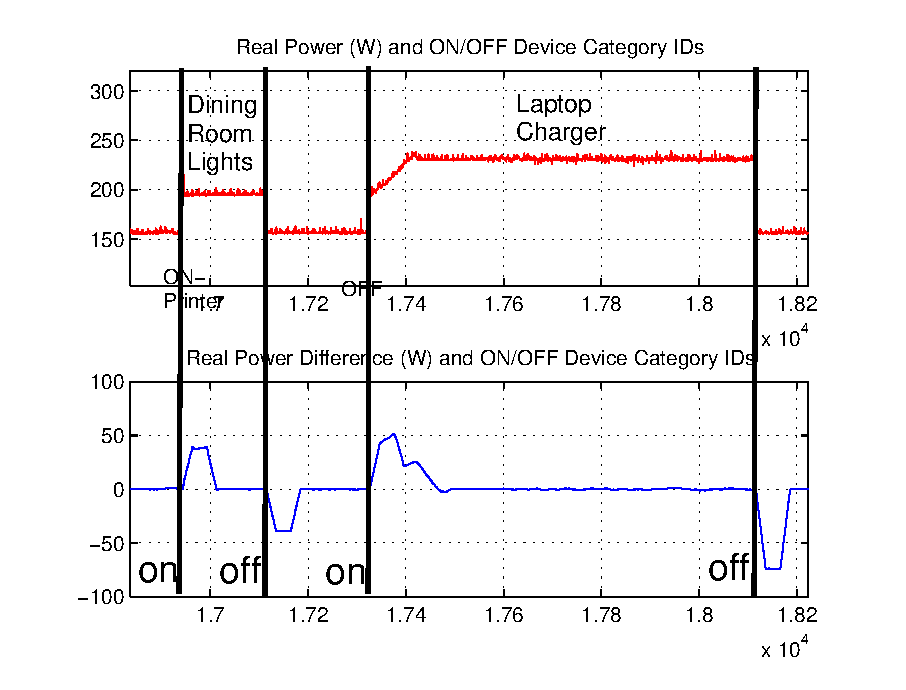
\includegraphics[width=3.5in]{fig/windowlength.eps}
	\caption{Simple Distribution Feeder.}
	\label{fig:windowlength}
\end{figure}

Cyclical loads exhibit unique characteristics throughout the entire operation.  Consider the dryer shown in Fig. \ref{fig:demon}.  The real power waveform consistently rises and falls until the appliance is turned off.  The turn-on and turn-off signature windows detect multiple events when there is actually a single event.  Therefore, in this case, the first-event captured by the turn-on window and the last-event captured by the turn-off windows should be paired up to detect this event.

Consider the oven shown in Fig. \ref{fig:demon}.  In addition to the turn-on signature window, 
additional window is extracted from the following real power jump.  




Outlier detection is also held in this stage.  Consider the four ON/OFF events of a computer as shown in Fig. \ref{fig:outlier}.  It is shown that when event 2 occurred, some background noise are introduced that affected the turn-on signature of the computer.  In this case, the second event is regarded as outliers and is not used in training the windows.

\begin{figure}[!t]
	\centering
	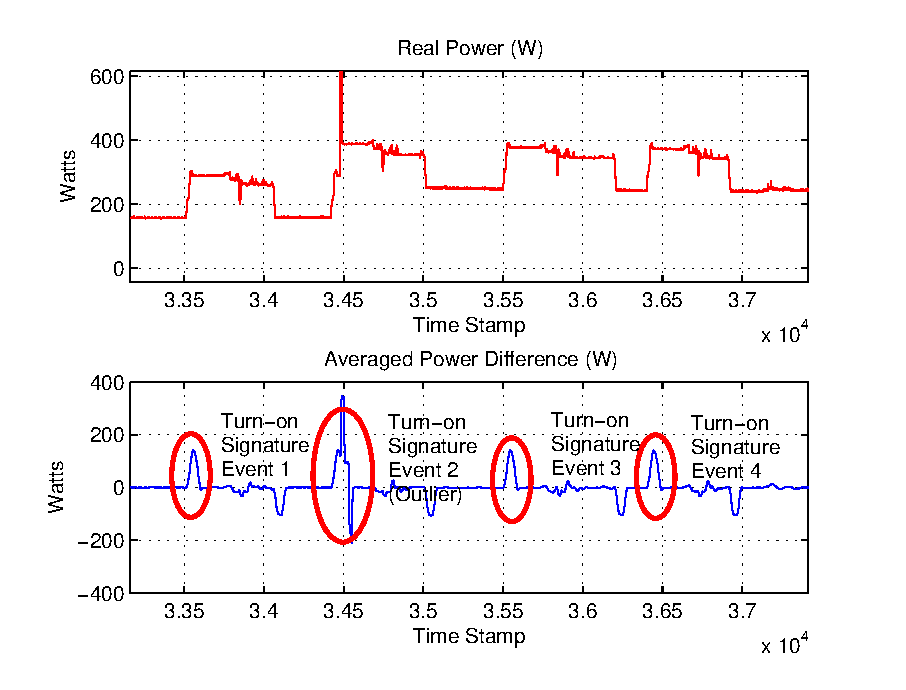
\includegraphics[width=3.5in]{fig/outlier.eps}
	\caption{Outlier.}
	\label{fig:outlier}
\end{figure}
\newpage
=======
%	\begin{figure}[!t]
%		\centering
%		\subfloat[]{\includegraphics[width=2.5in]{fig/event1.jpg}
%			\label{fig:event1}}
%		\hfil
%		\subfloat[]{\includegraphics[width=2.5in]{fig/event1.jpg}
%			\label{fig:event2}}
%		\caption{Fault Current Waveform (a) Original waveform, (b) Truncated waveform used for the study.}
%		\label{fig:demon}
%	\end{figure}	
	
	
%\begin{figure}[!t]
%	\centering
%	\subfloat[]{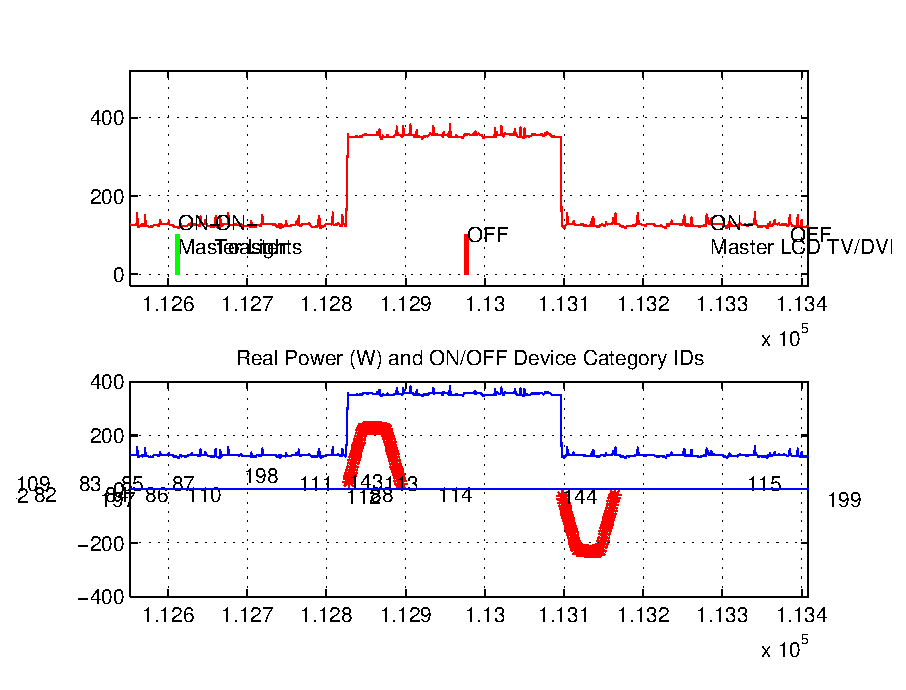
\includegraphics[width=2.5in]{fig/masterlights.eps}
%		\label{fig:rec}}
%\end{figure}

First a event detector is used in the real power domain to estimate the exact switching time of the event.  By  in the training data.  This is to account for the mismatches of the provided tagging info and the exact switching index.  

A typical rectangular load shape of is shown in Figure \ref{fig:rec}.  Many appliances turned out to have rectangular load shape and these appliances can be separated using real and reactive power consumption features.  Figure \ref{fig:PQ} shows feature space of appliances that have rectangular load shape.  The feature vector of each class are clustered together, implying that the real and reactive power features are sufficient for classifying most of the appliances.


This section concentrates on extracting the feature windows in low frequency data.  In particular the real and the reactive power differences are used to extract these windows.  First, a separate event detector is used to correct the   event detector is used in the Training Data to correct the mismatches 



The procedures for calculating the real power and the reactive power include event detection, data smoothing, and power calculation.

\subsection{Load Types}
-constant power - static 
	- resistive (lights, heaters, kettle) - P domain and rectangular mainly
	- resistive + reactive (rotating like fans) - Q is a feature to help classify
-dynamic
	- cyclical (washer dryer) - require rules, ie. landmark detection
>>>>>>> 4a1b9769f1a3f8f92b061559235daa35c859fc63
	
\subsubsection{Subsubsection Heading Here}
Subsubsection text here.


% An example of a floating figure using the graphicx package.
% Note that \label must occur AFTER (or within) \caption.
% For figures, \caption should occur after the \includegraphics.
% Note that IEEEtran v1.7 and later has special internal code that
% is designed to preserve the operation of \label within \caption
% even when the captionsoff option is in effect. However, because
% of issues like this, it may be the safest practice to put all your
% \label just after \caption rather than within \caption{}.
%
% Reminder: the "draftcls" or "draftclsnofoot", not "draft", class
% option should be used if it is desired that the figures are to be
% displayed while in draft mode.
%
%\begin{figure}[!t]
%\centering
%\includegraphics[width=2.5in]{myfigure}
% where an .eps filename suffix will be assumed under latex, 
% and a .pdf suffix will be assumed for pdflatex; or what has been declared
% via \DeclareGraphicsExtensions.
%\caption{Simulation Results.}
%\label{fig_sim}
%\end{figure}

% Note that IEEE typically puts floats only at the top, even when this
% results in a large percentage of a column being occupied by floats.


% An example of a double column floating figure using two subfigures.
% (The subfig.sty package must be loaded for this to work.)
% The subfigure \label commands are set within each subfloat command,
% and the \label for the overall figure must come after \caption.
% \hfil is used as a separator to get equal spacing.
% Watch out that the combined width of all the subfigures on a 
% line do not exceed the text width or a line break will occur.
%
%\begin{figure*}[!t]
%\centering
%\subfloat[Case I]{\includegraphics[width=2.5in]{box}%
%\label{fig_first_case}}
%\hfil
%\subfloat[Case II]{\includegraphics[width=2.5in]{box}%
%\label{fig_second_case}}
%\caption{Simulation results.}
%\label{fig_sim}
%\end{figure*}
%
% Note that often IEEE papers with subfigures do not employ subfigure
% captions (using the optional argument to \subfloat[]), but instead will
% reference/describe all of them (a), (b), etc., within the main caption.


% An example of a floating table. Note that, for IEEE style tables, the 
% \caption command should come BEFORE the table. Table text will default to
% \footnotesize as IEEE normally uses this smaller font for tables.
% The \label must come after \caption as always.
%
%\begin{table}[!t]
%% increase table row spacing, adjust to taste
%\renewcommand{\arraystretch}{1.3}
% if using array.sty, it might be a good idea to tweak the value of
% \extrarowheight as needed to properly center the text within the cells
%\caption{An Example of a Table}
%\label{table_example}
%\centering
%% Some packages, such as MDW tools, offer better commands for making tables
%% than the plain LaTeX2e tabular which is used here.
%\begin{tabular}{|c||c|}
%\hline
%One & Two\\
%\hline
%Three & Four\\
%\hline
%\end{tabular}
%\end{table}


% Note that IEEE does not put floats in the very first column - or typically
% anywhere on the first page for that matter. Also, in-text middle ("here")
% positioning is not used. Most IEEE journals/conferences use top floats
% exclusively. Note that, LaTeX2e, unlike IEEE journals/conferences, places
% footnotes above bottom floats. This can be corrected via the \fnbelowfloat
% command of the stfloats package.

 


\section{Cross-Validation-ML}
Discuss cross validation here. this is the whole procedure for generating thresholds.

need figures as examples of P/Q domain, diff domain, distance domain, window shape (big subplot 3x3?)

\section{Test Data}
- rules for on/off pairing

\section{Conclusion}
The conclusion goes here. All insight gained from competition. Too many appliances, noisy test data, what is the benefit of identifying small appliances?, noise necessitates clear features (large distance).  also high freqency domain for hard to identify appliances.  you can get 20th w/ just P/Q alone.   




% conference papers do not normally have an appendix


% use section* for acknowledgement
\section*{Acknowledgment}


The authors would like to thank...





% trigger a \newpage just before the given reference
% number - used to balance the columns on the last page
% adjust value as needed - may need to be readjusted if
% the document is modified later
%\IEEEtriggeratref{8}
% The "triggered" command can be changed if desired:
%\IEEEtriggercmd{\enlargethispage{-5in}}

% references section

% can use a bibliography generated by BibTeX as a .bbl file
% BibTeX documentation can be easily obtained at:
% http://www.ctan.org/tex-archive/biblio/bibtex/contrib/doc/
% The IEEEtran BibTeX style support page is at:
% http://www.michaelshell.org/tex/ieeetran/bibtex/
%\bibliographystyle{IEEEtran}
% argument is your BibTeX string definitions and bibliography database(s)
%\bibliography{IEEEabrv,../bib/paper}
%
% <OR> manually copy in the resultant .bbl file
% set second argument of \begin to the number of references
% (used to reserve space for the reference number labels box)

%\begin{thebibliography}{1}
%
%\bibitem{IEEEhowto:kopka}
%H.~Kopka and P.~W. Daly, \emph{A Guide to \LaTeX}, 3rd~ed.\hskip 1em plus
%  0.5em minus 0.4em\relax Harlow, England: Addison-Wesley, 1999.
%
%\end{thebibliography}

%\begin{thebibliography}{1}
%
%\end{thebibliography}

\bibliography{Bib}
\bibliographystyle{ieeetr}



% that's all folks
\end{document}


